\documentclass{beamer}
\usepackage{subfigure}
\usepackage{caption}

% There are many different themes available for Beamer. A comprehensive
% list with examples is given here:
% http://deic.uab.es/~iblanes/beamer_gallery/index_by_theme.html
% You can uncomment the themes below if you would like to use a different
% one:
%\usetheme{AnnArbor}
%\usetheme{Antibes}
%\usetheme{Bergen}
%\usetheme{Berkeley}
%\usetheme{Berlin}
%\usetheme{Boadilla}
%\usetheme{boxes}
%\usetheme{CambridgeUS}
%\usetheme{Copenhagen}
%\usetheme{Darmstadt}
%\usetheme{Frankfurt}
%\usetheme{Goettingen}
%\usetheme{Hannover}
%\usetheme{Ilmenau}
%\usetheme{JuanLesPins}
%\usetheme{Luebeck}
%\usetheme{Madrid}
%\usetheme{Malmoe}
%\usetheme{Marburg}
%\usetheme{Montpellier}
%\usetheme{PaloAlto}
%\usetheme{Pittsburgh}
%\usetheme{Rochester}
%\usetheme{Singapore}
%\usetheme{Szeged}
%\usetheme{Warsaw}

\title{Spatial Reading Group}

% A subtitle is optional and this may be deleted
\subtitle{Optional Subtitle}

%\date{Conference Name, 2013}
% - Either use conference name or its abbreviation.
% - Not really informative to the audience, more for people (including
%   yourself) who are reading the slides online

\subject{blah}
% This is only inserted into the PDF information catalog. Can be left
% out. 

% If you have a file called "university-logo-filename.xxx", where xxx
% is a graphic format that can be processed by latex or pdflatex,
% resp., then you can add a logo as follows:

% \pgfdeclareimage[height=0.5cm]{university-logo}{university-logo-filename}
% \logo{\pgfuseimage{university-logo}}

% Delete this, if you do not want the table of contents to pop up at
% the beginning of each subsection:
\AtBeginSubsection[]
{
  \begin{frame}<beamer>{Outline}
    \tableofcontents[currentsection,currentsubsection]
  \end{frame}
}

% Let's get started
\begin{document}

\begin{frame}
  \titlepage
\end{frame}

\begin{frame}{Outline}
  \tableofcontents
  % You might wish to add the option [pausesections]
\end{frame}

% Section and subsections will appear in the presentation overview
% and table of contents.
\section{Motivation}


\begin{frame}{Motivation}{Why Spatial Data needs Spatial Stats}
  \begin{itemize}
  \item {
    Spatial Data are continuous but measured discretely.
  }
  \item {
    The data tend to be correlated.
  }
  \item {
  	The measurements are rarely taken at random
    
  }
  \end{itemize}
\end{frame}

\begin{frame}{Assumptions}{}
  \begin{itemize}
  \item {
    Smooth data
  }
  \item {
    Stationary data
	\begin{itemize}
   		\item Does a trend extend beyond the bounds of the study?
   		\item Is the covariance consistent in the bounds of the study?
    \end{itemize}
  }
  \end{itemize}
\end{frame}

\section{Classical Frequentist Spatial Stats}
\subsection{Spatial Relationships}
\begin{frame}{Covariance}{}
  \begin{itemize}
  \item {
    Smooth data
  }
  \item {
    Stationary data
	\begin{itemize}
   		\item Does a trend extend beyond the bounds of the study?
   		\item Is the covariance consistent in the bounds of the study?
    \end{itemize}
  }
  \end{itemize}
\end{frame}

\begin{frame}{Mattern Function}{}
  \begin{itemize}
  \item { 
  		$\rho(x) =\{2^{\kappa-1} \Gamma(\kappa)\}^{-1} \frac{u}{\phi}^\kappa K_\kappa (\frac{u}{\phi})$
  }
  \item {
    $\kappa$ is order of differentiation, smoothness
  }
  \item{
  	$\phi is scale, degree of decay over time$
  }
  \item{
  	$\kappa$ and $\phi$ are not orthogonal.
  }
  \end{itemize}
\end{frame}

\subsection{Variograms}

% You can reveal the parts of a slide one at a time
% with the \pause command:
\begin{frame}{Second Slide Title}
  \begin{itemize}
  \item {
    First item.
    \pause % The slide will pause after showing the first item
  }
  \item {   
    Second item.
  }
  % You can also specify when the content should appear
  % by using <n->:
  \item<3-> {
    Third item.
  }
  \item<4-> {
    Fourth item.
  }
  % or you can use the \uncover command to reveal general
  % content (not just \items):
  \item<5-> {
    Fifth item. \uncover<6->{Extra text in the fifth item.}
  }
  \end{itemize}
\end{frame}


\begin{frame}{Kriging}
	\begin{itemize}
		
		\item Suppose our objective is to predict the value of the signal at an arbitrary location $S(x)$.
		
		\item Note that $(S(x), Y)$ is multivariate Gaussian with mean vector $\mu \mathbf{1}$ and covariance matrix
		$$
		\begin{pmatrix}
		\sigma^2 & \sigma^2 r^T\\
		\sigma^2 r & \sigma^2 V
		\end{pmatrix},
		$$
		where $r$ is a vector with elements $r_i = \rho(\|x-x_i\|)$ and $V = \sigma^2 R + \tau^2 I$.
		
		
	\end{itemize}
\end{frame}

\begin{frame}{Kriging}
	\begin{itemize}
		
		\item Conditional mean and variance:
		$$E(S(x) | Y) = \mu + r^T V^{-1}(Y - \mu \mathbf{1}),$$
		$$Var(S(x) | Y) = \sigma^2 (1 - r^T V^{-1} r).$$
		
		\item Two types:
		\begin{itemize} 
			\item Ordinary kriging: replace $\mu$ by its weighted least squares estimator
			$$\hat{\mu} = (\mathbf{1}^T V^{-1} \mathbf{1})^{-1} \mathbf{1}^T V^{-1} Y.$$
			
			\item Simple kriging: replace $\mu$ by $\hat{\mu} = \bar{y}$.
		\end{itemize}
		
		
		
		\item Both kriging predictors can be expressed as a linear combination: $\hat{S}(x) = \sum_{i=1}^{n}a_i(x) Y_i$, but $\sum_{i=1}^{n}a_i(x)=1$ only for ordinary kriging.
	\end{itemize}
\end{frame}

\begin{frame}{Maximum Likelihood Estimation}
	\begin{itemize}
		\item Gaussian model
		$$Y \sim N(D\beta, \sigma^2 R(\phi) + \tau^2I) $$
		with covariates matrix $D_{n\times p}$, regression coefficients $\beta$ ,  covariance of a parametric model for $S(x)$, and nugget variance $\tau^2$. 
		\item The log-likelihood function is 
		\begin{align*}
		L(\beta, \tau^2, \sigma^2, \phi) =  &- 0.5 \{n \log(2\pi) + log\{|(\sigma^2 R(\phi) +\tau^2 I) | \} \\
		&+ (y-D\beta)^T(\sigma^2 R(\phi) + \tau^2 I)^{-1} (y - D\beta)\}
		\end{align*}
		\item Let $\nu^2 = ({\tau^2} /{\sigma^2})$, $V = R(\phi) + \nu I$, then $L(\beta, \tau^2, \sigma^2, \phi)$ is maximized at 
		\begin{align}
		\hat{\beta}(V) &= (D^T V^{-1}D)^{-1}D^TV^{-1}y \\
		\hat{\sigma}^2(V) &= n^{-1} \{y - D\hat{\beta}(V)\}^T V^{-1}\{y - D\hat{\beta}(V)\} 
		\end{align}
	\end{itemize}
\end{frame}

\begin{frame}{Maximum Likelihood Estimation}
	\begin{itemize}
		\item Plug (1) and (2) into $L(\beta, \tau^2, \sigma^2, \phi)$ and obtain  the {\color{blue}concentrated log-likelihood}: 
		$L_0(\nu^2, \phi) = -0.5 \{n \log (2 \pi) + n \log \hat{\sigma}^2(V) +  log |V|+ n \}$
		\item Optimize $L_0(\nu^2, \phi)$ numerically with respect to $\nu$ and $\phi$; \\ back substitution to obtain $\hat{\sigma}^2$ and $\hat{\beta}$
		\item Re-parameterisation of $V$ can be used to obtain more stable estimation, e.g  the ratio $\sigma^2 / \phi$ is more stable than $\sigma^2$ and $\phi$
		\item  Computational tool:  {\color{blue}profile log-likelihood}: \\
		Assume a model with parameters $(\alpha, \psi)$, 
		$$L_p(\alpha) = L(\alpha, \hat{\psi}(\alpha))  = \max_{\psi}(L(\alpha, \psi))$$  %. help to calculation CI for each individual parameter; Full maximum likelihood estimation then requires numerical maximisation  jointly. 
	\end{itemize}
\end{frame}

\begin{frame}{Maximum Likelihood Estimation}
	\begin{itemize}
		\item Non-Gaussian data: \\ 
		(1): transformation to Gaussian (2)  generalized linear model 
		\item   (1) E.g. Box-Cox transformation; denote the transformed responses $Y^{\ast} = (Y_1^{\ast}, ..., Y_n^{\ast})$, and fit a Gaussian model 
		$$Y^{\ast} \sim N(D\beta, \sigma^2 \{R(\phi) + \tau^2I\}) $$
		Computationally demanding, transformation may impede scientific interpretation
		\item (2) Generalized linear model 
		\begin{align*}  %notations book page 123, may need to explain theta and g , no space on this slide : ( ...
		L(\theta|S) &= \prod_{i=1}^n f_i(y_i|S, \theta)\\
		L(\theta, \phi) &= \int_ S \prod_{i=1}^n f_i(y_i|s, \theta)g(s|\phi) ds
		\end{align*}
		Involve high dimensional integration;need MCMC/Hierarchical likelihood/Generalized estimating equations
	\end{itemize}
\end{frame}


\begin{frame}{Maximum Likelihood Estimation (An Example)} %not sure if we want this slide, elevation data on page 115
	\begin{figure}
		\centering
		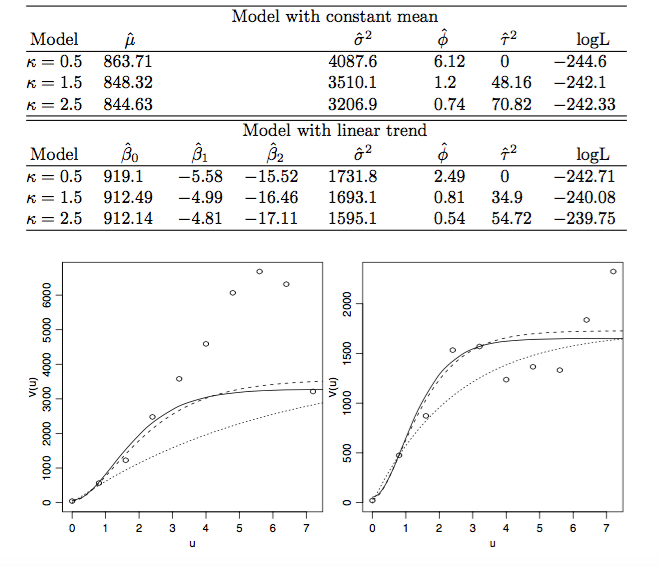
\includegraphics[scale = 0.35]{Images/Pic1}
		\captionsetup{font={small,it}}
		\caption{ { \scriptsize left: constant mean model; right: linear trend surface \newline  circle: sample  variogram; solid line $\kappa = 2.5$; dashed line $\kappa = 1.5$; dotted line $\kappa = 0.5$}}
	\end{figure}
\end{frame}

\section{Extension - Preferential Sampling}

\begin{frame}{Preferential Sampling}
\begin{block}{The Problem}
\begin{itemize}
\item So far we have assumed the sampling locations $X$ are fixed, or assumed known.
\item What if the sampling locations depend on the underlying field $S$?
\end{itemize}
\end{block}

\begin{example}
\begin{itemize}
\item Pollution data from measuring stations
\item Ocean temperature data from marine mammals
\item Lead concentration in Galicia (to be shown)
\end{itemize}
\end{example}
\end{frame}

\begin{frame}{Preferential Sampling}

\begin{figure}
\centering
\caption{Example of a single realisation of $S$ and corresponding 100 sampling locations selected using a spatial Poisson Process with intensity $\lambda(x)=\exp(\beta S(x))$.\label{fig:PrefSimPlot}}
\subfigure[Example of 100 preferentially sampled locations ($\beta=2$)]{\label{fig:a}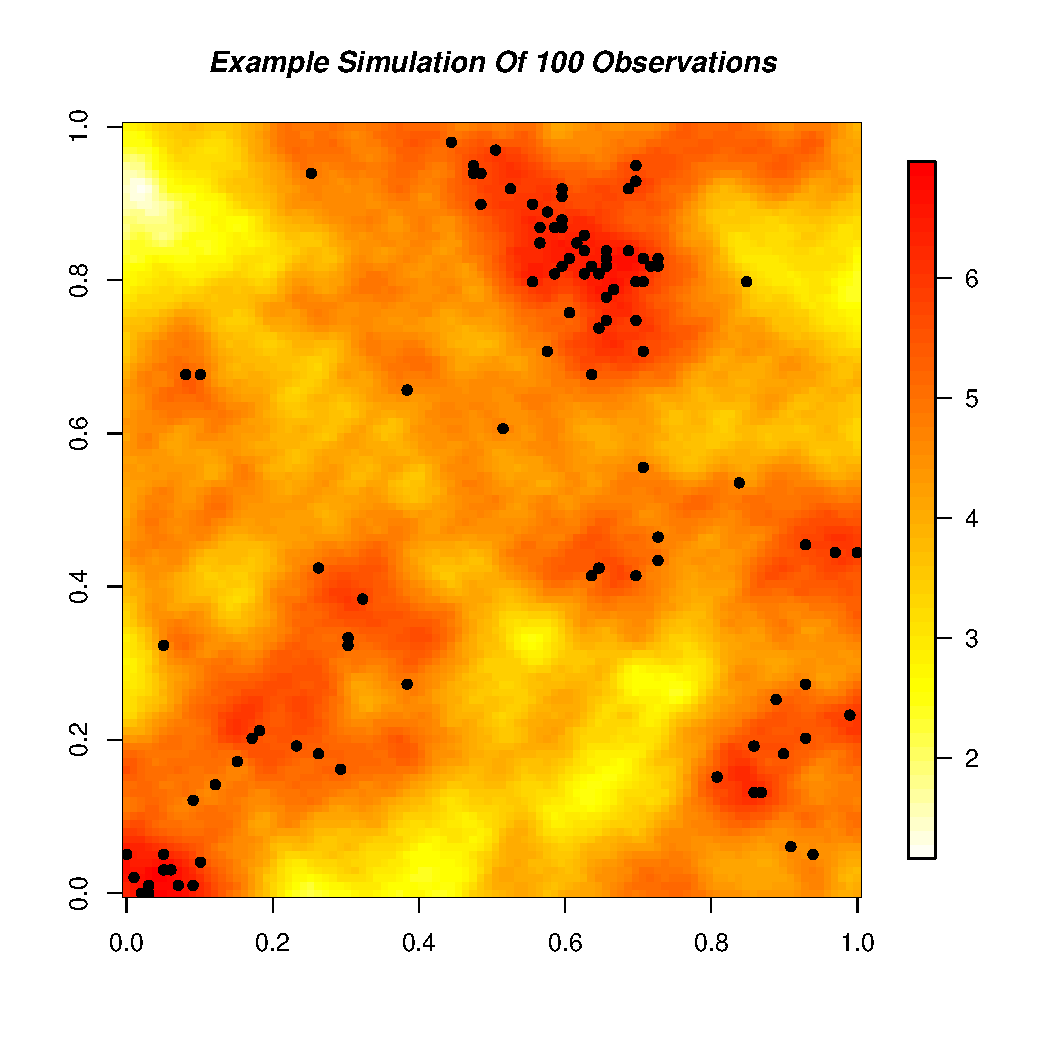
\includegraphics[width=50mm]{Images/DiggleFakeSimPlot.pdf}}
\subfigure[Example of 100 non-preferentially sampled locations ($\beta=0$)]{\label{fig:b}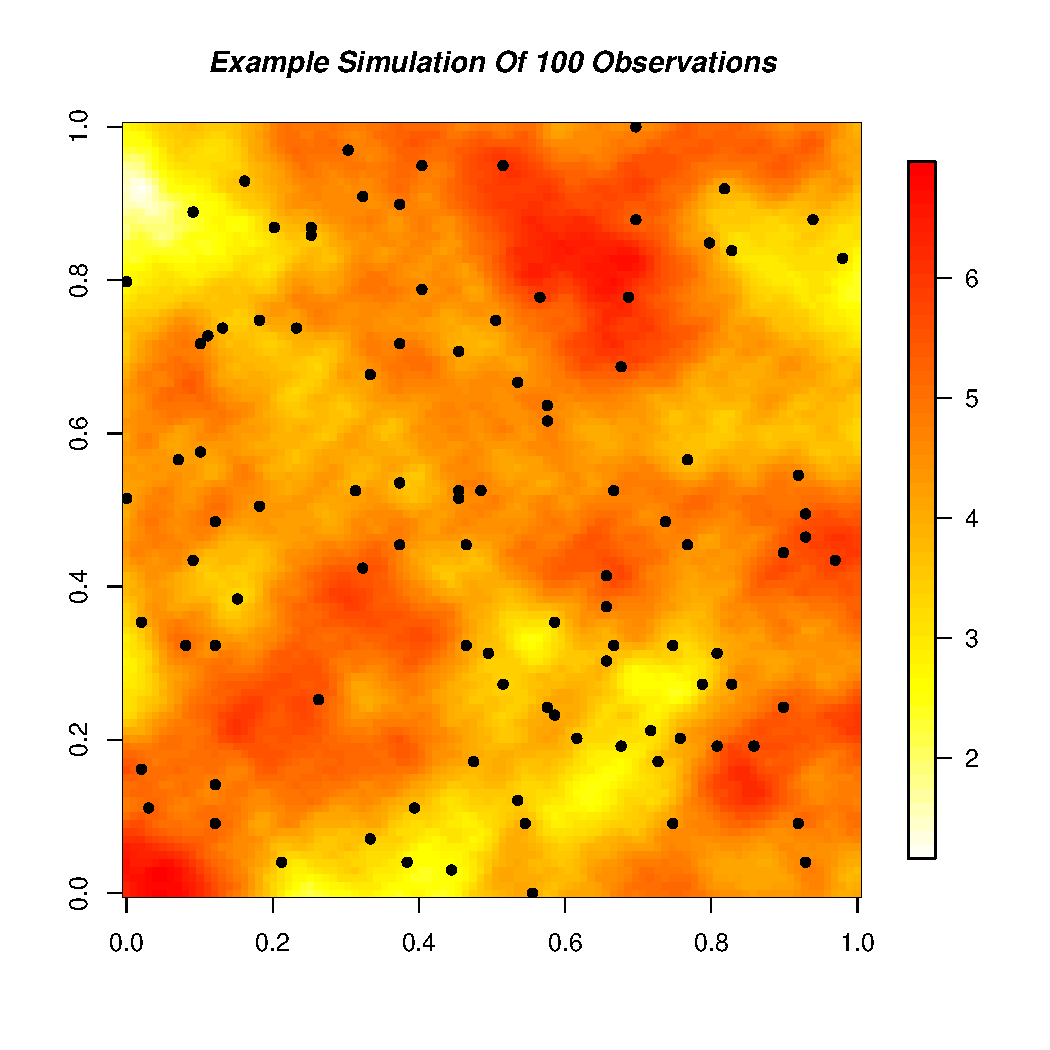
\includegraphics[width=50mm]{Images/DiggleFakeSimPlotNP.pdf}}
\end{figure}
\end{frame}

\begin{frame}{Preferential Sampling}
\begin{block}{Solution}
\begin{itemize}
\item We must account for the dependence between $X$ and $S$.
\begin{equation}
L(\boldsymbol{\theta})=\int \left[X,Y,S\right]\mathrm{d}S.
\end{equation}
\item Diggle et al. 2010 - Monte Carlo 
\item Integrated Nested Laplace Approximation (INLA) - Joe
\item Template Model Builder - Danny
\end{itemize}
\end{block}
\end{frame}

\begin{frame}{Preferential Sampling}
\begin{block}{Results}
\small
\begin{table}[ht]
\centering
    \begin{tabular}{| c | c | c | c | c |}
    \hline
    Model & Parameter  & Standard MLE & {\it TMB} \\ \hline
    Preferential & Bias & (0.77, 1.36)  & (0.41, 0.94) \\
    Preferential & Root-mean-square error & (0.86, 1.40) & (0.60, 1.05)  \\ \hline
\end{tabular}
    \caption {Comparison of approximate $95\%$ confidence intervals for the root-mean-square errors and bias between standard MLE and {\it TMB} over 50 independent simulations for preferential ($\beta=2$) at location $x_0=(0.49, 0.49)$.}
 \label{table:simtable}
\end{table}
\normalsize
\end{block}

\end{frame}

\section{Bayesian Estimation and Prediction}

\begin{frame}{Problems with the MLE approach}

\begin{itemize}
\item MLE method seperates parameter estimation and spatial prediction as two distinct problems.
\item First the model is formulated, and it's parameters estimated.
\item These estimated parameters are assumed true and spatial prediction equations are computed with these estimates plugged-in.
\item Parameter uncertainty is ignored when making spatial prediction.
\item Parameter uncertainty is often VERY HIGH. Even with seemingly large datasets ($n > 10,000$), the positive correlation dilutes the information present. Largely different values of correlation parameters $\phi$ often fit the data equally well.
\end{itemize}

\end{frame}

\begin{frame}{Bayesian approach}

\begin{itemize}
\item Account for parameter uncertainty when making spatial prediction and hence make more conservative estimates of prediction accuracy.
\end{itemize}

\begin{align*}
[S | Y ] = \int [S | Y, \theta ] [ \theta | Y ] d \theta
\end{align*}

\begin{itemize}
\item The Bayesian predictive distribution is a weighted average of plug-in predictive distributions $[S | Y, \hat{\theta} ]$, weighted by the posterior uncertainty of the model values $\theta$.
\item Arbitrary nonlinear functional $T(S)$ of $S$ can be estimated (along with credible intervals, standard errors etc) by simple deterministic transformations of the posterior samples of $S$.
\end{itemize}

\end{frame}

\begin{frame}{Problems with Bayesian implementation}

\begin{itemize}
\item Due to the flexibility of the Matern correlation function, many different combinations of the correlation parameters $\phi$ fit the data equally well.
\item A consequence of this is that the posterior distribution of $[\theta | Y]$ has non-negligible probability mass across a wide range of the parameter space.
\item The first consequence of this is that posterior distributions are extremely sensitive to prior distributions. Apparently 'diffuse' priors can still heavily affect the location and scale of the posterior distribution.
\item Secondly, MCMC samplers must be formulated with large transition jumps to ensure the whole parameter space is explored. This leads to VERY LONG MCMC chains needing to be run (100,000 +).
\end{itemize}

\end{frame}

\begin{frame}{The joy of INLA}

\begin{itemize}
\item INLA enables \textbf{very} accurate deterministic approximations to both $[\theta | Y]$ and $\int [S | Y, \theta ] [ \theta | Y ] d \theta$ to be obtained.
\item INLA handles most well-known response functions (Binomial, Poisson, Gamma etc), enabling Generalized Geostatistical Models to be fit.
\item Through a combination of high-accuracy Laplace approximations and cubic spline interpolation, values from INLA are often indistinguishable from the 'true' values from an MCMC chain.
\item INLA is FAST. Taking only seconds - minutes to run compared with the hours - days that MCMC can take. 
\item Multiple responses can be fit to the same spatial process! (E.g poisson process and intensity process enabling preferential sampling to be investigated.)
\end{itemize}

\end{frame}

\begin{frame}{Real example: Predicting total Tin in Cornwall, UK}
\begin{block}{Sampled data}
Please insert bubble plot
\end{block}

\end{frame}

\begin{frame}{Real example: Predicting total Tin in Cornwall, UK}
\begin{block}{Predicted field}
Please insert predicted mean field
\end{block}

\end{frame}

\begin{frame}{Real example: Predicting total Tin in Cornwall, UK}
\begin{block}{Upper and lower 95\% credible field}
Please insert side-by-side 95\% credible interval field
\end{block}
\end{frame}
% Placing a * after \section means it will not show in the
% outline or table of contents.
\section*{Summary}

\begin{frame}{Summary}
  \begin{itemize}
  \item
    The \alert{first main message} of your talk in one or two lines.
  \item
    The \alert{second main message} of your talk in one or two lines.
  \item
    Perhaps a \alert{third message}, but not more than that.
  \end{itemize}
  
  \begin{itemize}
  \item
    Outlook
    \begin{itemize}
    \item
      Something you haven't solved.
    \item
      Something else you haven't solved.
    \end{itemize}
  \end{itemize}
\end{frame}



% All of the following is optional and typically not needed. 
\appendix
\section<presentation>*{\appendixname}
\subsection<presentation>*{For Further Reading}

\begin{frame}[allowframebreaks]
  \frametitle<presentation>{For Further Reading}
    
  \begin{thebibliography}{10}
    
  \beamertemplatebookbibitems
  % Start with overview books.

  \bibitem{Author1990}
    A.~Author.
    \newblock {\em Handbook of Everything}.
    \newblock Some Press, 1990.
 
    
  \beamertemplatearticlebibitems
  % Followed by interesting articles. Keep the list short. 

  \bibitem{Someone2000}
    S.~Someone.
    \newblock On this and that.
    \newblock {\em Journal of This and That}, 2(1):50--100,
    2000.
  \end{thebibliography}
\end{frame}

\end{document}
